\chapter[La biologie structurale au sein d'environnements immersifs et interactifs]{Contexte et état de l'art}
\minitoc
\cleardoublepage

\section{Liste des figures}

\begin{itemize}
	\item Cristallographie à différentes résolutions
\end{itemize}

\section{La biologie structurale et l'outil informatique}

L'étude des différents métabolismes régulant la vie des cellules, unité de base constituant l'ensemble des organismes vivants, peut être divisée en plusieurs sous-domaines caractérisés par l'échelle à laquelle les phénomènes sont observés, par la nature des organismes étudiés et par les méthodes utilisés pour les étudier. Parmi ces sous-domaines, la biologie moléculaire s'intéresse à l'étude de la structure et des interactions entre biomolécules (ADN, ARN et protéines) et leur synthèse au sein de la cellule. Elle a pour but d'expliquer des phénomènes biologiques de grandes échelles d'un point de vue moléculaire. La biologie moléculaire se rapproche beaucoup de la biochimie à qui elle emprunte plusieurs techniques et idées. La biochimie s'intéresse à l'étude des phénomènes chimiques régissant les interactions entre les biomolécules. Autre discipline gravitant autour de l'étude des interactions, fonctions et structures des molécules, la biophysique possède une approche plus quantitative de la question et cherche à expliquer les phénomènes moléculaires grâce aux lois physiques régissant le reste du monde. A l'intersection de ces trois domaines d'études se trouve la biologie structurale, domaine spécifiquement intéressé aux structures mêmes des biomolécules, aux étapes permettant à une biomolécule d'acquérir une structure fonctionnelle et aux effets de la structure sur la fonction des biomolécules. C'est un domaine d'étude utilisant plusieurs techniques expérimentales, principalement de biophysiques, afin d'obtenir une description de précision atomique de la structure des molécules étudiées et de leur dynamique structurelle dans leur environnement cellulaire, impliquant donc les interactions qu'elles peuvent avoir avec d'autres biomolécules et la conséquence sur leur structure, et donc leur fonction.

\subsection{Techniques expérimentales}

Les techniques expérimentales utilisées en biologie structurale pour obtenir la structure tertiaire de biomolécules sont relativement coûteuses de part leur complexité. En effet, les techniques de microscopie optique standards ne peuvent permettre aujourd'hui une observation à l'échelle atomique, quel que soit l'objet d'étude. Ce sont donc des méthodes physiques indirectes qui sont principalement utilisées afin d'obtenir des informations sur la structure 3d d'une biomolécule à l'échelle atomique. La plupart de ces techniques mettent en jeu des instruments de mesure de haute technologie et parfois une préparation complexe de l'échantillon nécessitant un effort scientifique important.

\subsubsection{Cristallographie à rayons X ou radiocristallographie}

Parmi ces techniques expérimentales, la plus ancienne et la plus utilisée, principalement pour sa précision, est la cristallographie aux rayons X ou radiocristallographie. Cette technique consiste à envoyer un faisceau de rayons X sur un cristal composé exclusivement de la biomolécule étudiée. La mesure des angles et de l'intensité des rayons réfractés permet d'obtenir une image tridimensionnelle de la densité électronique dans le cristal. A partir de cette densité, il est possible d'obtenir la position moyenne des atomes présents dans le cristal ainsi que les liens existants entre-eux en superposant la séquence d'atomes, connue, dans la carte de densité électronique ainsi obtenue. 
L'avantage de la radiocristallographie est sa très grande précision et l'absence de limite de taille pour le cristal, permettant l'observation de structures moléculaires de très grande taille comme les ribosomes (environ un million d'atomes). Suivant les biomolécules observées, il est possible d'obtenir des structures tridimensionnelles à des résolutions comprises entre 2 et 3\r{A} (Angströms = \SI{e-10}{\metre}) pour une précision sur la position des atomes autour de 0.5\r{A}. 1\r{A} de résolution permet une précision atomique quasi-parfaite. Les cartes de densité et les modèles atomiques créés à partir de ces cartes sont illustrés dans la figure X. 
Certaines biomolécules sont néanmoins très difficiles à cristalliser et on évalue à environ un quart la proportion de macromolécules permettant de créer un cristal de taille et de qualité suffisante de diffracter suffisamment les rayons X. Cette cristallisation est une étape peu facilement automatisable et qui se révèle majoritairement empirique, demandant un travail spécifique en plus de l'application de la technique. Les hydrogènes présents dans les macromolécules sont très difficiles à percevoir du fait de leur très faible densité électronique.

\subsubsection{Spectroscopie à Résonance Magnétique Nucléaire (RMN)}

Également très utilisée, la RMN consiste à envoyer une séquence précise d'impulsions électromagnétiques sur une molécule en présence d'un champ magnétique. La fréquence et la séquence des impulsions électromagnétiques sont propres à chaque type d'atome. Cette technique se base sur les mouvements de rotation naturels des atomes, créant un mini champ magnétique (ou spin). Seuls quelques atomes sont adaptés à la spectroscopie RMN car ils possèdent un spin nucléaire de 1/2. En biologie structurale, c'est principalement le proton H\textsuperscript{1} qui est ciblé. Les noyaux atomiques possédant des spins sont excités par les impulsions électromagnétiques et absorbent l'énergie ainsi reçue. Lors de l'étape de relaxation suivant l'impulsion, les noyaux atomiques relâchent de l'énergie sous forme de résonance à différentes longueurs d'onde, calculée et reportée par les instruments de mesure. Cette résonance varie en fonction de la nature de l'atome excité et de son environnement. Il est donc possible, grâce à ces résonances, pour un atome donné, d'avoir des informations sur la nature et le nombre d'atomes voisins, la liaison chimique dans laquelle il est impliqué, sa distance à d'autres atomes, sa mobilité, etc... A la différence de la cristallographie, la RMN peut s'appliquer sur une solution composée de la molécule étudiée et il est de fait plus aisé de stabiliser une molécule en solution que de la cristalliser. Il est également possible d'avoir des informations sur la dynamique de la molécule puisqu'au contraire de quand elle se trouve dans un cristal, une molécule en solution n'est pas statique.
L'état dynamique de la molécule est aussi un inconvénient pour obtenir une structure 3d fixe puisque la précision de la mesure sera perturbée par les changements structurels de la molécules. L'un des autres inconvénients de la spectroscopie RMN est la taille des molécules observée du fait de la complexité du traitement des signaux de résonance magnétique, ces derniers se superposant sur un spectre de largeur fixe. Ainsi, plus le nombre d'atome est important, plus le nombre de signaux augmentera et s'accumulera sur un spectre de largeur constante. La taille optimale pour la RMN varie entre 10 et 50 kilo-Dalton (kDa) correspondant à des molécules de 1.500 à 10.000 atomes. de plus, Pour les plus grosses molécules, il est nécessaire d'effectuer un marquage isotopique permettant d'obtenir un spectre non plus 2d mais 3d où les atomes ciblés, en plus de H\textsuperscript{1}, sont le C\textsuperscript{13} et le N\textsuperscript{15} après enrichissement spécifique de la biomolécule observée.

\subsubsection{Cryo-microscopie électronique}

Autre technique populaire en biologie structurale, la cryo-microscopie électronique consiste à utiliser le principe de la microscopie électronique, et donc d'utiliser un faisceau de particules d'électrons au lieu de rayonnements électromagnétiques comme en microscopie optique, sur un échantillon préalablement cryogéniser lors de l'étape de fixation. Le faisceau de particule d'électrons passe au travers de lentilles électrostatiques et électromagnétiques puis au travers de l'échantillon où il est modifié pour former une image électronique finalement amplifiée par d'autres lentilles et projetée sur un scintillateur. 
La particularité de la cryofixation de l'échantillon, par opposé à la fixation chimique ou la déshydratation, est que l'échantillon est amené très rapidement à la température de l'azote liquide (\SI{-195.79}{\degreeCelsius}) ou de l'hélium liquide (\SI{-269}{\degreeCelsius}) afin que la glace formée ne soit pas cristalline et que le spécimen étudié conserve son état naturel. Pour des biomolécules, cela assure une conservation d'une structure 3d stable de la molécule. La cryo-EM permet d'étudier des structures moléculaires de grandes tailles, à partir de 300kDa jusqu'à des tissus de plusieurs centaines de nanomètres, en passant par les ribosomes, les virus ou les composants cellulaires.
Bien qu'en constante développement, la cryo EM possède une résolution relativement faible comparée aux deux techniques précédentes puisque les cartes de densité obtenues par cette technique ne permettent pas une résolution de moins de 4\r{A} pour les cartes les plus précises\cite{zhou_atomic_2011}. L'exposition de l'échantillon à un faisceau de particules d'électrons, combiné à sa cryogénisation, dommage significativement l'échantillon qui ne peut être réutilisé ensuite.

\subsubsection{Diffusion des rayons X - SAXS}

La technique SAXS est basée sur les interactions élastiques entre les photons et les nuages électroniques. Cette technique s'inspire directement de la diffraction des rayons X quand ils traversent un cristal (diffraction de Bragg) entraînant la diffusion de ces rayons à différents angles de l'ordre de la dizaine de degrés. L'angle de diffraction est inversement proportionnel à la distance interatomique des atomes présents dans le cristal. Or, les informations nécessaires pour constituer la structure 3d de macromolécules concernent des distances trop grandes pour que les angles de diffraction soient facilement détectables. Il est nécessaire d'utiliser un rayonnement X monochromatique très proche de l'échantillon constitué de la biomolécule d'intérêt.De la même manière que pour les précédentes techniques, une carte de densité, ici densité électronique, est ainsi générée après interprétation des angles de diffraction calculés par l'instrument de mesure placé à la suite du faisceau émis à travers l'échantillon.
L'un des avantages de la technique SAXS par rapport à la cristallographie est l'absence de cristal pour effectuer l'expérience, l'échantillon étant mis en solution. Mais cet avantage est terni par la résolution de la technique qui ne permet pas d'avoir une description atomique d'une biomolécule. Elle est souvent utilisée pour obtenir une structure 3d approximative de complexes moléculaires ou de composants cellulaires de grandes tailles. Une de ces forces repose aussi sur la rapidité de l'expérience qui, en combinant l'ensemble des étapes de préparation, expérimentation et analyses des résultats, peut générer une carte de densité en quelques jours.


En complément des analyses expérimentales possibles aujourd'hui, l'apport des approches computationnelles est conséquente. La puissance de calcul des outils informatiques permettent désormais d'intégrer des paramètres physico-chimiques à toute simulation numérique cherchant à créer des modèles 3d cohérents de biomolécules à partir de la simple séquence, ou enchaînement, de groupements moléculaires. Le fossé préalablement existant entre la précision des 

\subsection{Structure d'une protéine}

\subsection{Simulation moléculaire}

\subsection{Outils bioinformatiques}

\subsubsection{Visualisation moléculaire}

\subsubsection{Analyses et interprétation de simulations}

\section{Réalité virtuelle et interactivité}

\subsection{Immersion pour les données scientifiques}

\subsection{Paradigmes d'interaction en immersion}

\section{Visualisation analytique}

\subsection{Visualisation analytique interactive pour les données scientifiques}

\subsection{Représentation des connaissances}

\subsubsection{Bio-ontologies}

\cite{schulze-kremer_ontologies_2002}

\subsubsection{Web sémantique et formalismes à base de graphes}

Sesame [55] est une architecture générique pour le stockage persistant de RDF(S) dans une base de données et l'interrogation de ce RDF(S) avec le langage RQL. RQL [56] est un langage de requête RDF défini par le moyen d'un ensemble de requêtes fondamentales, un ensemble de filtres de base et un moyen de construire de nouvelles requêtes par une composition fonctionnelle et des itérateurs. Lors de l'analyse d’une requête RQL, Sesame construit une requête optimisée évaluée au moyen d'une série d'appels à la couche de stockage et d’inférence de Sesame.

Par comparaison RDQL [56] permet l'interrogation de données RDF au niveau de la structure, tandis que Sesame permet l’interrogation au niveau sémantique. En ce sens notre objectif est beaucoup plus proche de Sesame. Toutefois Sesame ne considère pas la sémantique des XSD datatypes, ni ne permet d’avoir des règles d'inférence exploitant les ontologies.

Jena [57] est l’un des moteurs actuels les plus complets et propose une persistance en mémoire ou en base de données. Il implante RDF, RDFS et OWL ainsi que les requêtes SPARQL et propose un moteur en chaînage avant (RETE), arrière (programmation logique) et hybride. Ce moteur est utilisé pour implanter la sémantique de RDFS et OWL. Le modèle de Jena repose sur une structure prédéfinie de bases de données.

Triple [58] est un langage de requêtes pour divers modèles de données du web sémantique. Le noyau Triple est un langage de requête RDF fondé sur la logique de Horn étendue par des fonctionnalités syntaxiques pour intégrer des primitives RDF comme les espaces de nommage, les ressources et les réifications. Ce langage peut être compilé en logique de Horn et exécuté par des moteurs Prolog. Triple n'est pas limité à l'interrogation de données RDF. Il dispose d'une architecture en couche lui permettant d'interroger d’autres modèles de données avec différents types de sémantique (ex : RDFS et DAML + OIL) et en ce sens il rejoint notre certitude qu’il faut abstraire les structures et algorithmes des différents langages que nous manipulons. Le noyau de Triple est étendu par des règles pour l’axiomatisation de la sémantique de RDFS ; elles peuvent être utilisées avec un moteur d'inférence pour dériver des connaissances supplémentaires à partir d'un schéma RDFS.

DAMLJessKB [59] et son successeur OWLJessKB ainsi que le cœur du eWallet [13] sont des outils de raisonnement pour DAML [60] ou OWL Lite. Ils ont tous les trois intégré JESS [61] un moteur de règles de production qu’ils appliquent à la sémantique de RDF, RDFS, DAML, XSD (XML Schema Datatypes [62]) et OWL Lite. Ils implantent une traduction des triplets RDF vers des faits du langage CLIPS de Jess et utilisent des règles de production pour décrire la sémantique des langages traduits. A l'aide de Jess, ces systèmes peuvent effectuer des raisonnements sur les classes et les instances.

OntoBroker [63] et son successeur On2broker sont des pionniers des systèmes à base d'ontologies basés sur les Frame Logics. OntoBroker gère des métadonnées intégrées dans des documents HTML avec des balises tout comme On2Brocker gère des annotations RDF. Dans les deux systèmes, les ontologies et les requêtes sont exprimées en langage frame logics qui permet la représentation d'une hiérarchie de types de concepts, d'une hiérarchie de types de relations et de règles. Le moteur de requête traduit ces représentations en Logique de Horn pour répondre à une requête.

OntoBroker, On2Broker, DAMLJessKB, OWLJessKB et partagent avec notre initiative le même principe général et les expressivités de leurs langages de représentation à base d’ontologie sont comparables. Toutefois, ces systèmes sont dédiés à des capacités générales de raisonnement sans exploiter les structures de graphes par exemple pour optimiser des opérations spécifiques à la recherche d'informations. Leurs langages de requêtes sont proches des logiques sur lesquelles ils se basent et restent dans leurs limites.

WebKB [64] [65] est un pionnier des serveurs web d'ontologies et des robots web basés sur les graphes conceptuels. Sur la base de sa simplicité et de l'exhaustivité de sa représentation, ses auteurs rejettent l'utilisation directe des langages basés sur XML. WebKB interprète et traduit automatiquement en graphes conceptuels des déclarations exprimées dans une notation linéaire des graphes et intégrées à des documents web. WebKB fournit des commandes de requête pour interroger les propriétés lexicales ou structurelles des documents HTML ou afficher des spécialisations ou généralisations d'un concept, d'une relation ou d'un graphe.

OntoSeek [66] est un autre système conçu pour la recherche d’information basée sur le contenu de pages jaunes et de catalogues de produits en ligne. Il combine les graphes conceptuels et des ontologies du domaine correspondant. Il met l'accent sur les contraintes lexicale et sémantique dans le codage des ressources en graphes conceptuels et la construction de requêtes. Requêtes et annotations des ressources sont des graphes conceptuels lexicaux entre lesquels on cherche des homomorphismes.

WebKB, OntoSeek et la plate-forme que nous spécifierons en section 3.3.4 partagent le même type de représentation à base de graphes, par conséquent, le même principe d’homomorphisme correspondant à une requête sur les graphes d'annotation en prenant en compte la subsomption des types de concepts et des types de relations. Mais ni WebKB ni OntoSeek n’intègre RDF(S) ou les règles dans leur représentation à base d’ontologie.

Avec la standardisation de OWL DL, les moteurs à base de logiques de descriptions ont pris une importance particulière. Citons : Fact et son successeur Fact ++ [67], KAON2 [68] (une branche de KAON qui lui est resté focalisé sur RDFS), Racer [69], Pellet [70]. Ces moteurs offrent des opérations classiques en logiques de descriptions : identification, classification, validation. L’interrogation se limite en général à des requêtes conjonctives et les mécanismes d’interrogation ne sont pas prévus pour exploiter la structure des graphes ni accepter des graphes de grande taille.

En conclusion, aucune des contributions citées ci-dessus ne cherche à mettre en place un modèle pivot et une plate-forme ouverte et open-source pour implanter efficacement les aspects des représentations relevant des graphes. Elles sont toutes liées à un langage particulier (le plus souvent une logique) et/ou à une application particulière.

En ce qui concerne les outils permettant de raisonner avec des graphes conceptuels, les deux principaux outils sont : CoGITaNt [71] développé conjointement par le LIRMM et le LERIA, plate-forme dédiée à la mise en œuvre de mécanismes de raisonnement sur les graphes conceptuels spécifiquement ; et Amine (développé par l'INSEA au Maroc), plate-forme dédiée au développement de systèmes intelligents, qui repose sur une combinaison de Prolog et de graphes conceptuels. Citons également Prolog+CG basé sur un précurseur d'Amine, à usage éducatif.

Corese [72] [73] [5] [74] est un moteur de recherche sémantique basé sur les graphes conceptuels. Il implante RDF/S et SPARQL et il est développé dans l’équipe Acacia puis Edelweiss. Plus précisément, il implante la sémantique de RDF, RDFS, ainsi que les datatypes, les propriétés transitives, symétriques et inverses de OWL Lite.

Comme le montre la Figure 31, CORESE combine les avantages d'utiliser le langage RDF(S)/XML pour exprimer et échanger des méta-données, et les mécanismes de requête et d'inférence disponibles pour le formalisme des Graphes Conceptuels.
% \begin{eqnarray}
% \left\{ \begin{array}{ll}
% 	F_1(V\!E=0.8)=&F1 \\
% 	F_1(V\!E=0.6)=&0.925F1\\
% 	F_1(V\!E=1.0)=&1.075F1\\
% \end{array} \right.
% \end{eqnarray}

% \begin{eqnarray}
% F_1(V\!E)=
% \left\{
% 	\begin{array}{lll}
% 		&(0.7+0.375 \cdot V\!E) \cdot F1& \mbox{ si $V\!E\geq0.6$}\\
% 		&0.925 \cdot F1& \mbox{ si $V\!E<0.6$}\\
% 	\end{array}
% \right.
% \end{eqnarray}

% \begin{equation} 
% \begin{split}
% b_{TL} & = 1 - \nu + \sqrt{\nu^2-1}\\
% \nu    & = 1-\frac{1}{\eta} \\
% \eta   & = \frac{10^{TL/10}-1}{\cos(2\pi\frac{3000}{F_e})-1}
% \end{split} 
% \end{equation} 

% \begin{eqnarray} 
% \vert H( e^{2i \pi fc /F_e}) \vert = \frac{\vert H(1) \vert}{ \sqrt[]{2}}  \label{Eqa:1}
% \end{eqnarray}


% \noindent En élevant au carré (\ref{Eqa:1}), on obtient :
 
% \begin{eqnarray} 
% 	\frac{b_{TL}^2}{2 \cdot (1-b_{TL})(1-\cos(2i \pi f_c / F_e)) + b_{TL}^2} &=& \frac{1}{2}
% \end{eqnarray}



% \begin{figure}
%   \centering
%   \subfloat
%   [{\it Sans dépendance}]
%   {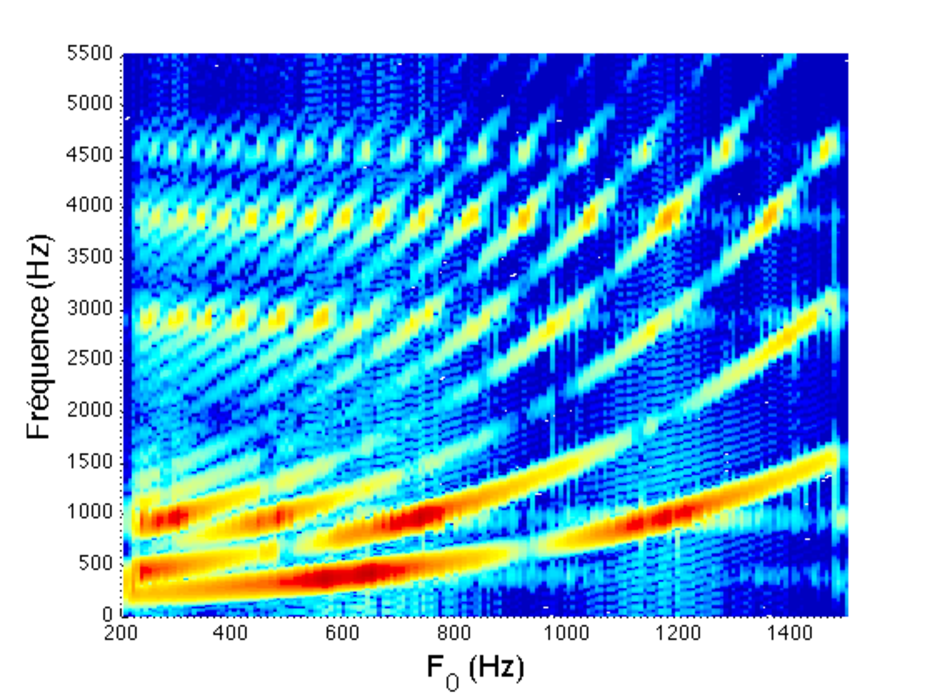
\includegraphics[width=.45\linewidth]{ch2/fig/Fi-F0-dpdce-sans_soprano_u_200-1500Hz_dig13b3.pdf}}
%   \label{Fig:Fi-F0-dpdce_sans}
%   \hspace{0.3cm}
%   \subfloat
% 	[{\it Avec dépendances}]  
%   {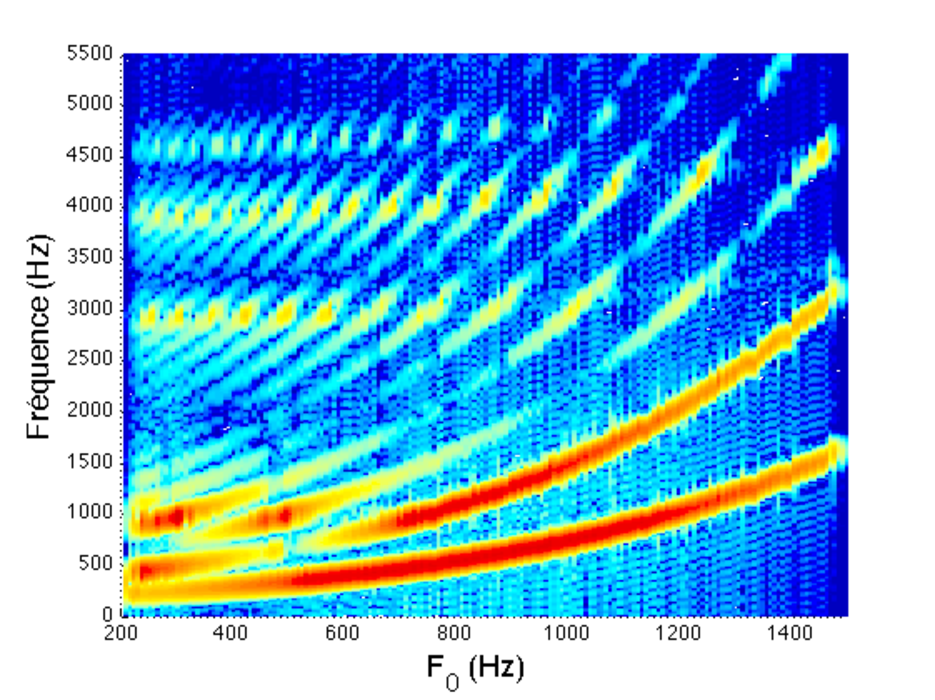
\includegraphics[width=.45\linewidth]{ch2/fig/Fi-F0-dpdce-avec_soprano_u_200-1500Hz_dig13b3.pdf}}
%   \label{Fig:Fi-F0-dpdce_avec}
%     \caption{{\it Spectrogrammes de la voyelle /a/ de synthèse, où $F_0$ augmente avec le temps, (a) sans ou (b) avec les dépendances entre les fréquences centrales des formants et de $F_0$. \textit{Voir fichiers audios~/ vidéos~\ref{fav:fi-f0-dependance}}\\
% }}
%   \label{Fig:Fi-F0-dpdce}
% \end{figure}

% \subsubsection{a) La soufflerie}

% \begin{table}[!h]
% 	\centering
% 	\begin{tabular}{|c|c|c|} 
% 		\hline
% 		& \centering \textbf{Tessiture naturelle moyenne} & \centering \textbf{Tessiture
% dans le synthétiseur} \tabularnewline
% 		\hline
% 		\bf Basse & Mi2-Mi4 & Sol$\sharp$1-Sol4\\
% 		\hline
% 		\bf Ténor & Do3-Si4 & Sol$\sharp$1-Sol4\\
% 		\hline
% 		\bf Alto & Fa3-Mi5 & Sol$\sharp$2-Sol5\\
% 		\hline
% 		\bf Soprano & Si3-Do6 & Sol$\sharp$3-Sol6\\
% 		\hline
% 	\end{tabular}
% 	\caption{\textit{Tessiture des chanteurs naturels et synthétiques (La3=440 Hz). Voir fichiers audios~/ vidéos~\ref{fav:types-voix-1}}}
% 	\label{Tab:tessChant}
% \end{table}

